\section{QOC for the Fluxonium \label{sec:fluxonium}}
In the following, we optimize quantum gates
(unitary transformations) for the fluxonium qubit.
The fluxonium is a promising building block
for quantum computers, and the accurate
two-level approximation of its Hamiltonian makes
QOC on a classical computer inexpensive.
In the two-level
approximation, the Hamiltonian takes the form:
\begin{align}
  H/h &= f_{q} \frac{\sigma_{z}}{2} + a(t) \frac{\sigma_{x}}{2}
  \label{eq:hamiltonian}
\end{align}
where $f_{q}$ is the qubit frequency at the flux frustration point,
$a(t)$ is the flux-drive amplitude, $h$ is Planck's constant, and $\sigma_{z}, \sigma_{x}$
are Pauli matrices. We optimize $X/2$, $Y/2$, and
$Z/2$ gates for the fluxonium presented in \cite{zhang2020universal},
and compare them to the analytically constructed gates for
that device.

First, we outline the constraints for the fluxonium gate problem.
We formulate this problem as a multi-state-transfer problem.
The initial conditions on
the states are $\ket{\psi^{0}_{1}} = \ket{0}$, $\ket{\psi^{1}_{1}} = \ket{1}$
\eqref{eq:istate_con}
where the superscript is an index $i \in \{0, 1\}$,
and the subscript indicates the first knot point $k = 1$.
The states at the final knot point are constrained to be
the image of the initial states under the desired gate $U$,
$\ket{\psi^{i}_{N}} = U \ket{\psi^{i}_{1}} \ \forall \ i$
\eqref{eq:tstate_con}.
%% This constraint is sensitive to global phase
%% differences between the states.
%% , but it is computationally efficient
%% because the Jacobian and Hessian
%% of the corresponding constraint function are diagonal.
%% We could have analogously chosen a metric which is insensitive
%% to global phases, such as the fidelity of the states.
Furthermore, we impose the normalization constraint
${\lvert \braket{\psi^{i}_{k}}{\psi^{i}_{k}} \rvert}^{2} = 1 \ \forall \ i,k$
\eqref{eq:statenorm_con}
to ensure the solver does not take advantge of discretization errors in numerical integration.
To refer to the discrete moments the flux amplitude, we introduce the notation
$\int^{t_{k}}_{t_{1}} a(t) \ \mathrm{d}t \equiv \int_{t} a_{k}$,
$a(t) \lvert_{t = t_{k}} \equiv a_{k}$,
$\pdv*[n]{a(t)}{t} \lvert_{t = t_{k}} \equiv \partial^{n}_{t} a_{k}$.
We impose the zero net flux constraint $\int_{t} a_{N} = 0$
\eqref{eq:znf_con}
which mitigates the hysteresis ubiquitous in flux-bias lines
\cite{battistel2019fast, krantz2019quantum, zhang2020universal}.
The flux amplitude is constrained by $\lvert a_{k} \rvert \leq 0.5 \ \textrm{GHz} \ \forall \ k$
\eqref{eq:amp_con}
to ensure the two-level approximation \eqref{eq:hamiltonian} remains valid.
We also enforce the boundary condition $a_{1} = a_{N} = 0$ \eqref{eq:bound_con}
so the gates may be concatenated arbitrarily. Additionally,
we have the initial condition $\int_{t} a_{1} = \partial_{t} a_{1} = 0$
\eqref{eq:ic_con}.

%% F1
\begin{figure*}[ht]
  
  \begin{subfigure}{.315\textwidth}
    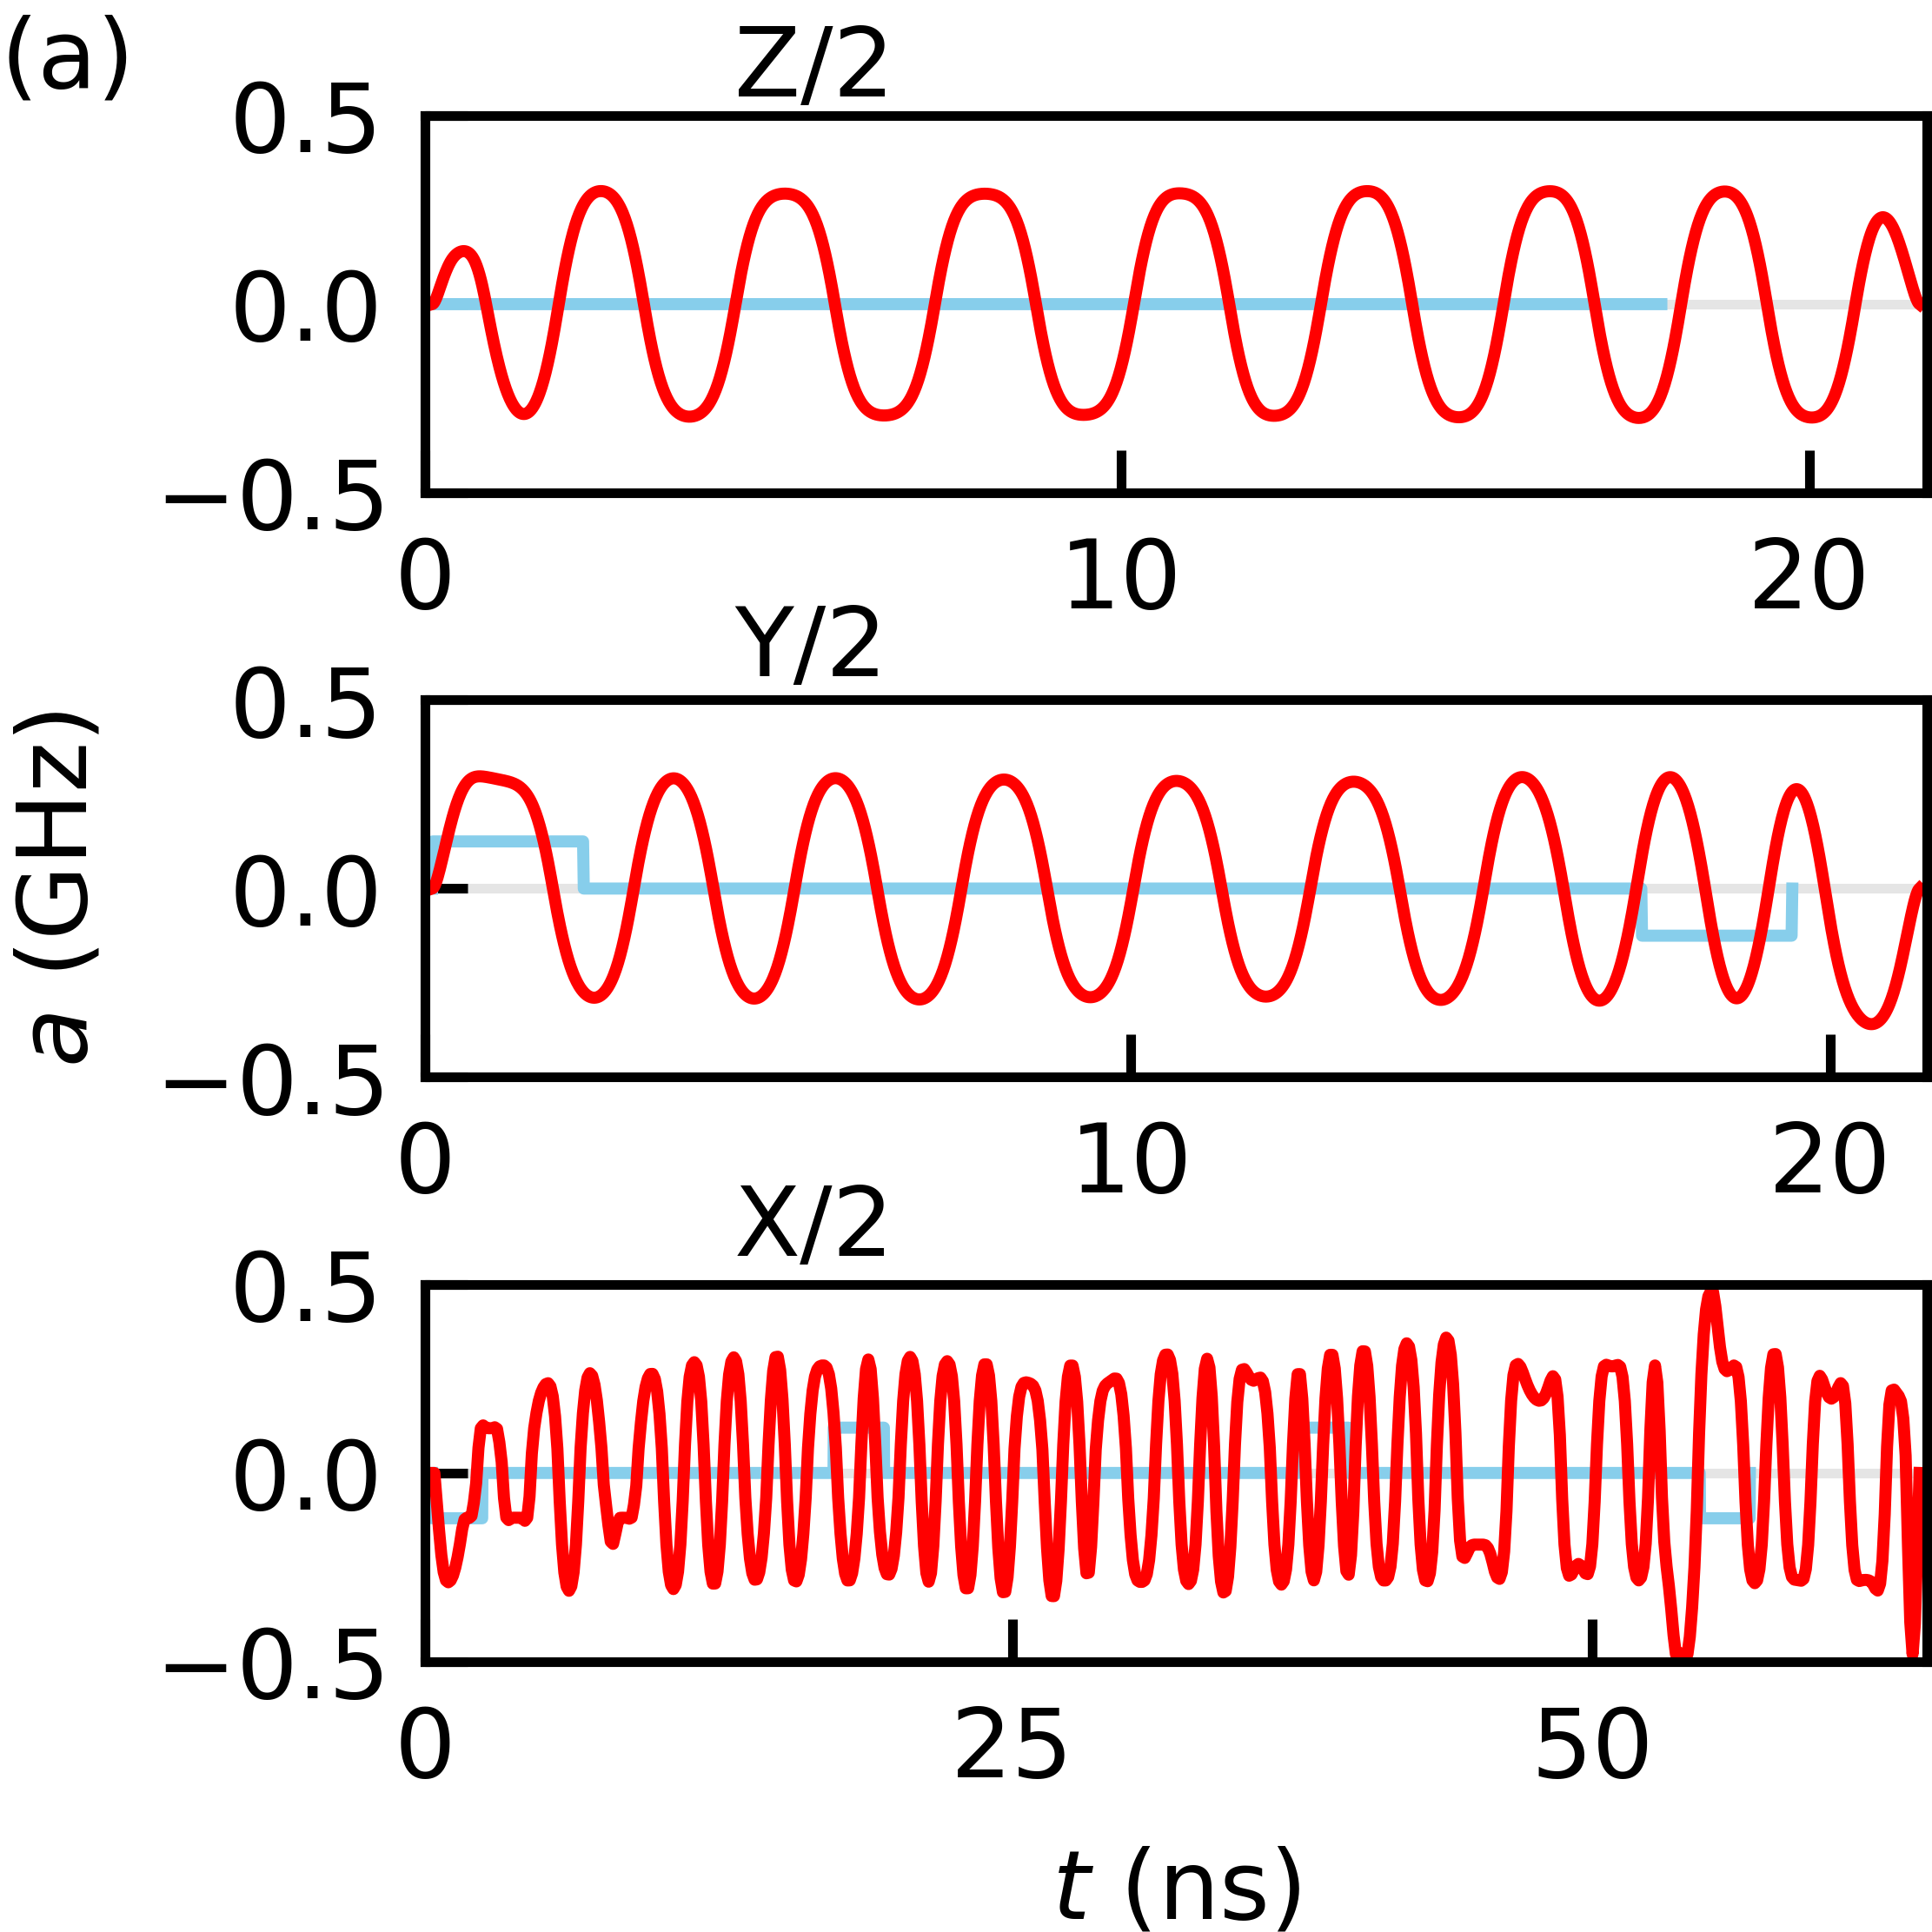
\includegraphics[width=\linewidth]{assets/f1a.png}
    \caption{\label{fig:longitudea}}
  \end{subfigure}\hfill
  \begin{subfigure}{.23\textwidth}
    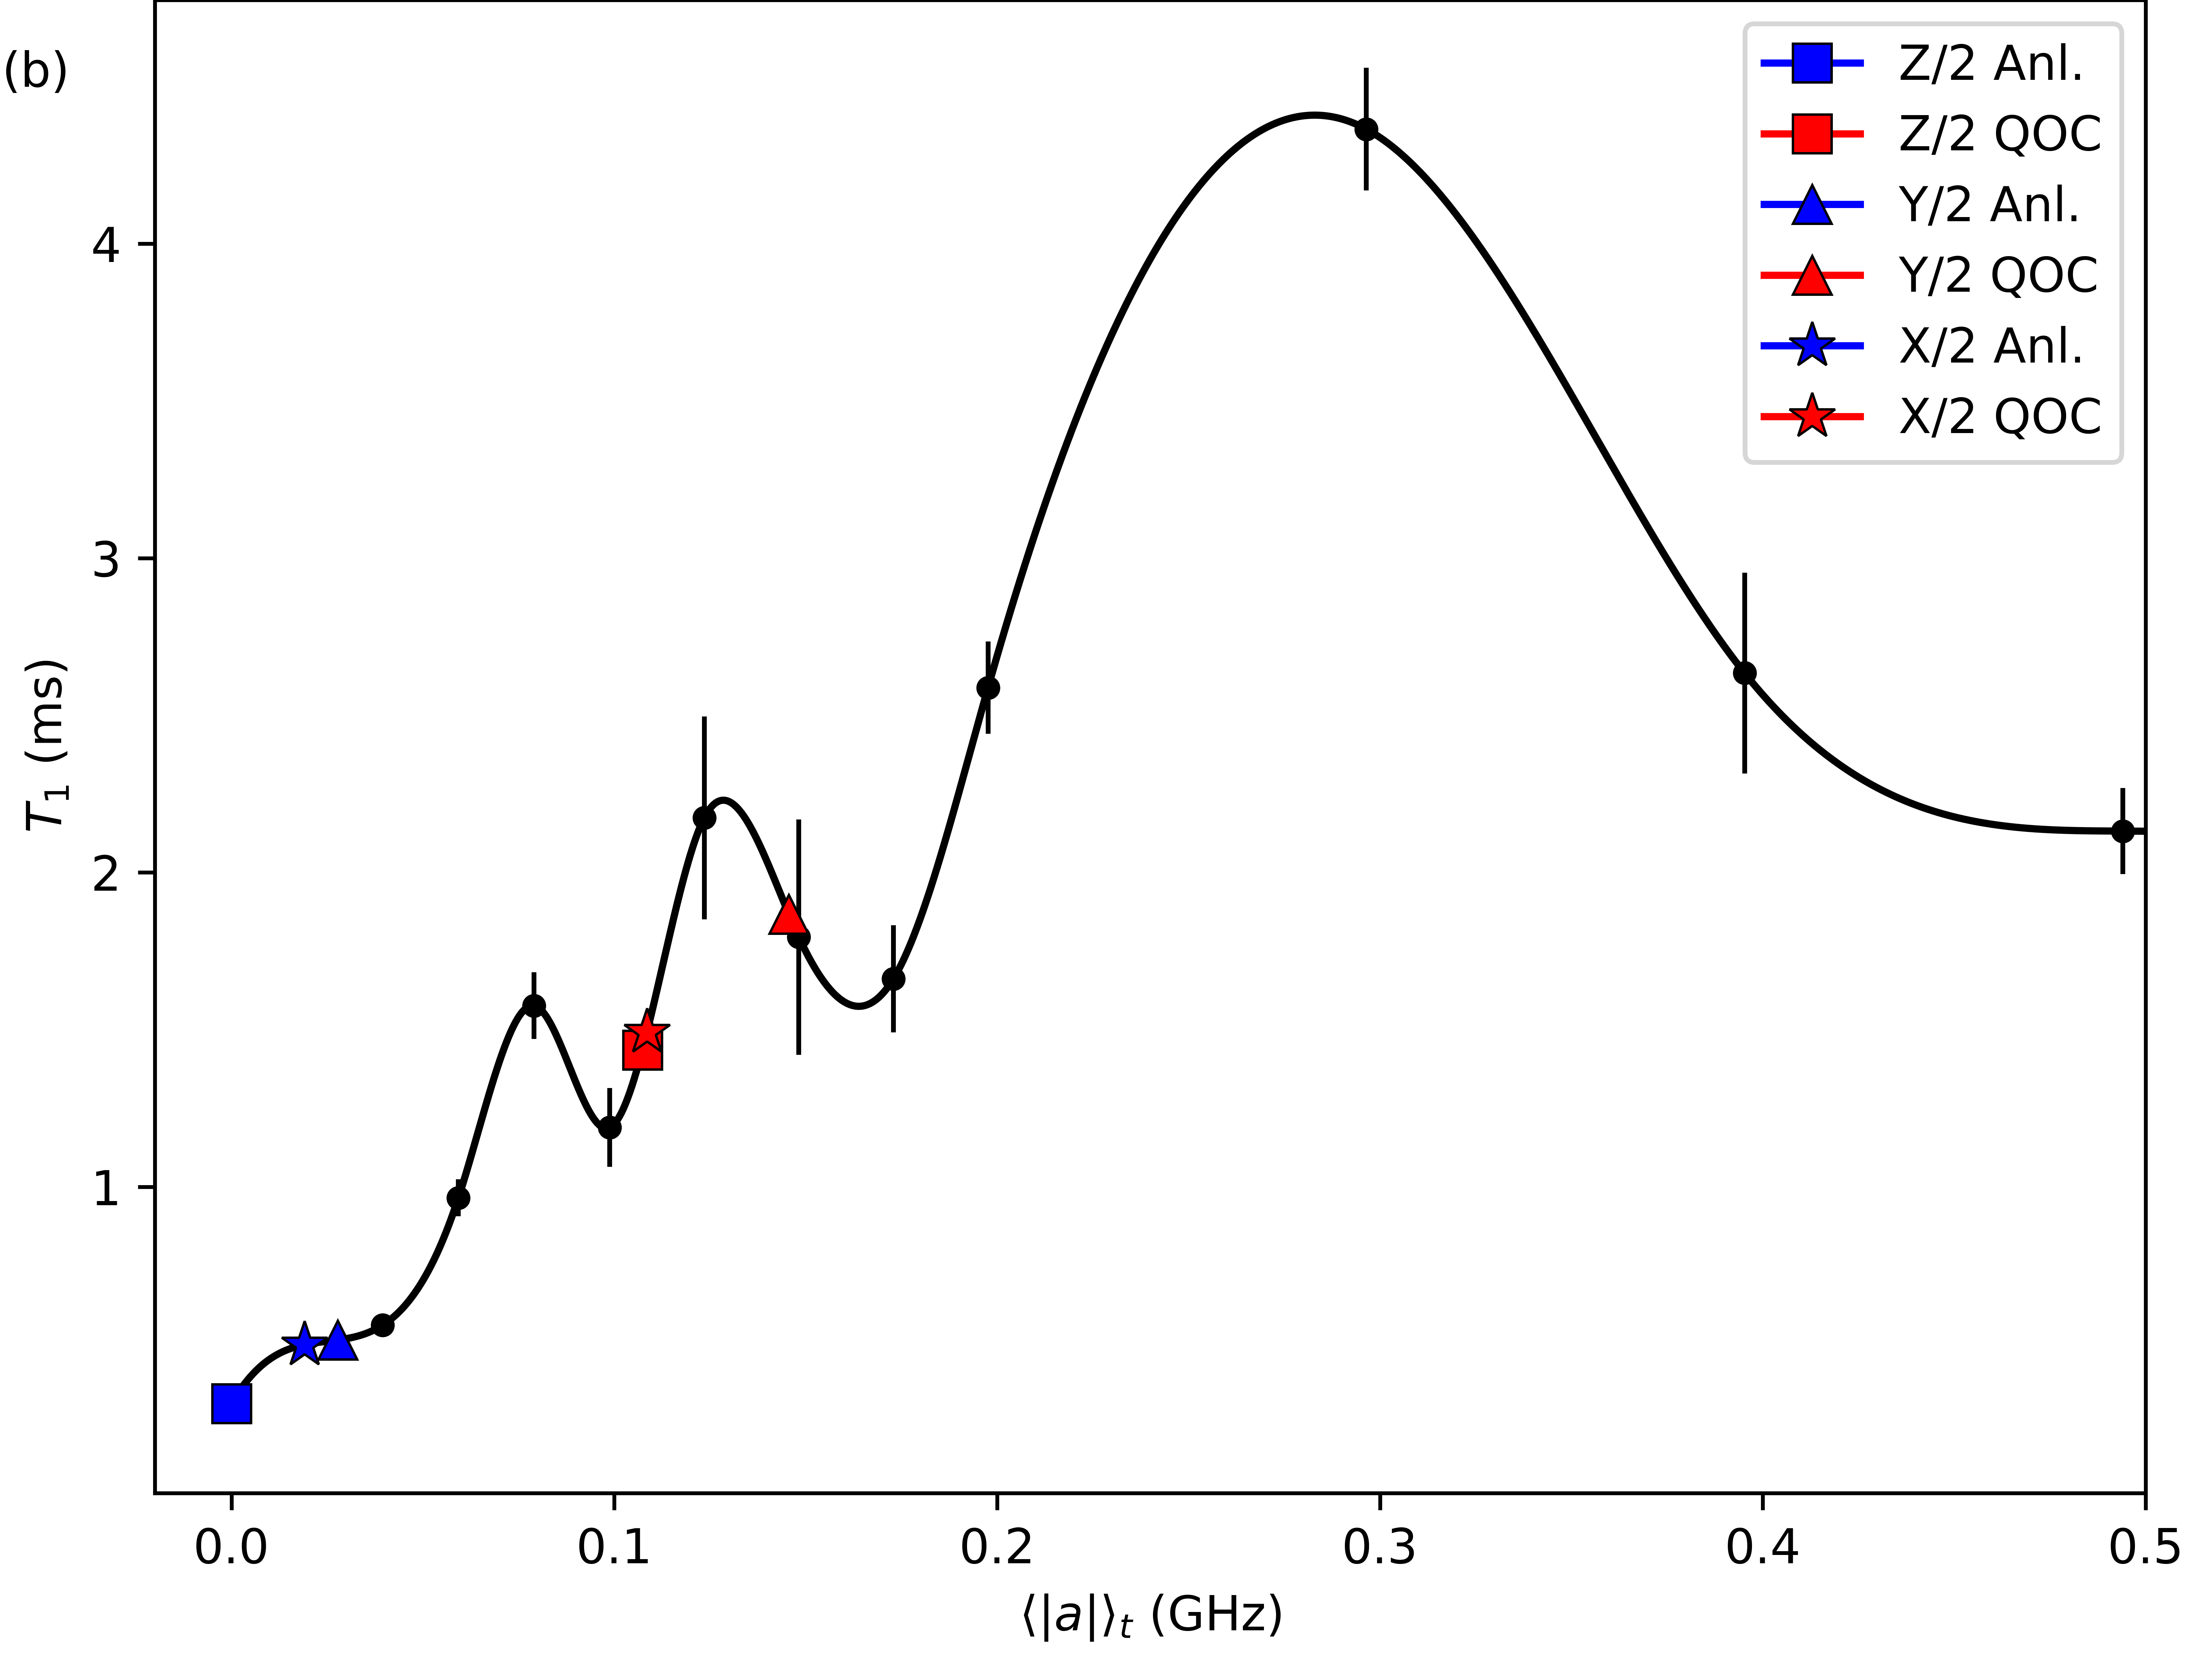
\includegraphics[width=\linewidth]{assets/f1b.png}
    \caption{\label{fig:longitudeb}}
  \end{subfigure}\hfill
  \begin{subfigure}{.4\textwidth}
    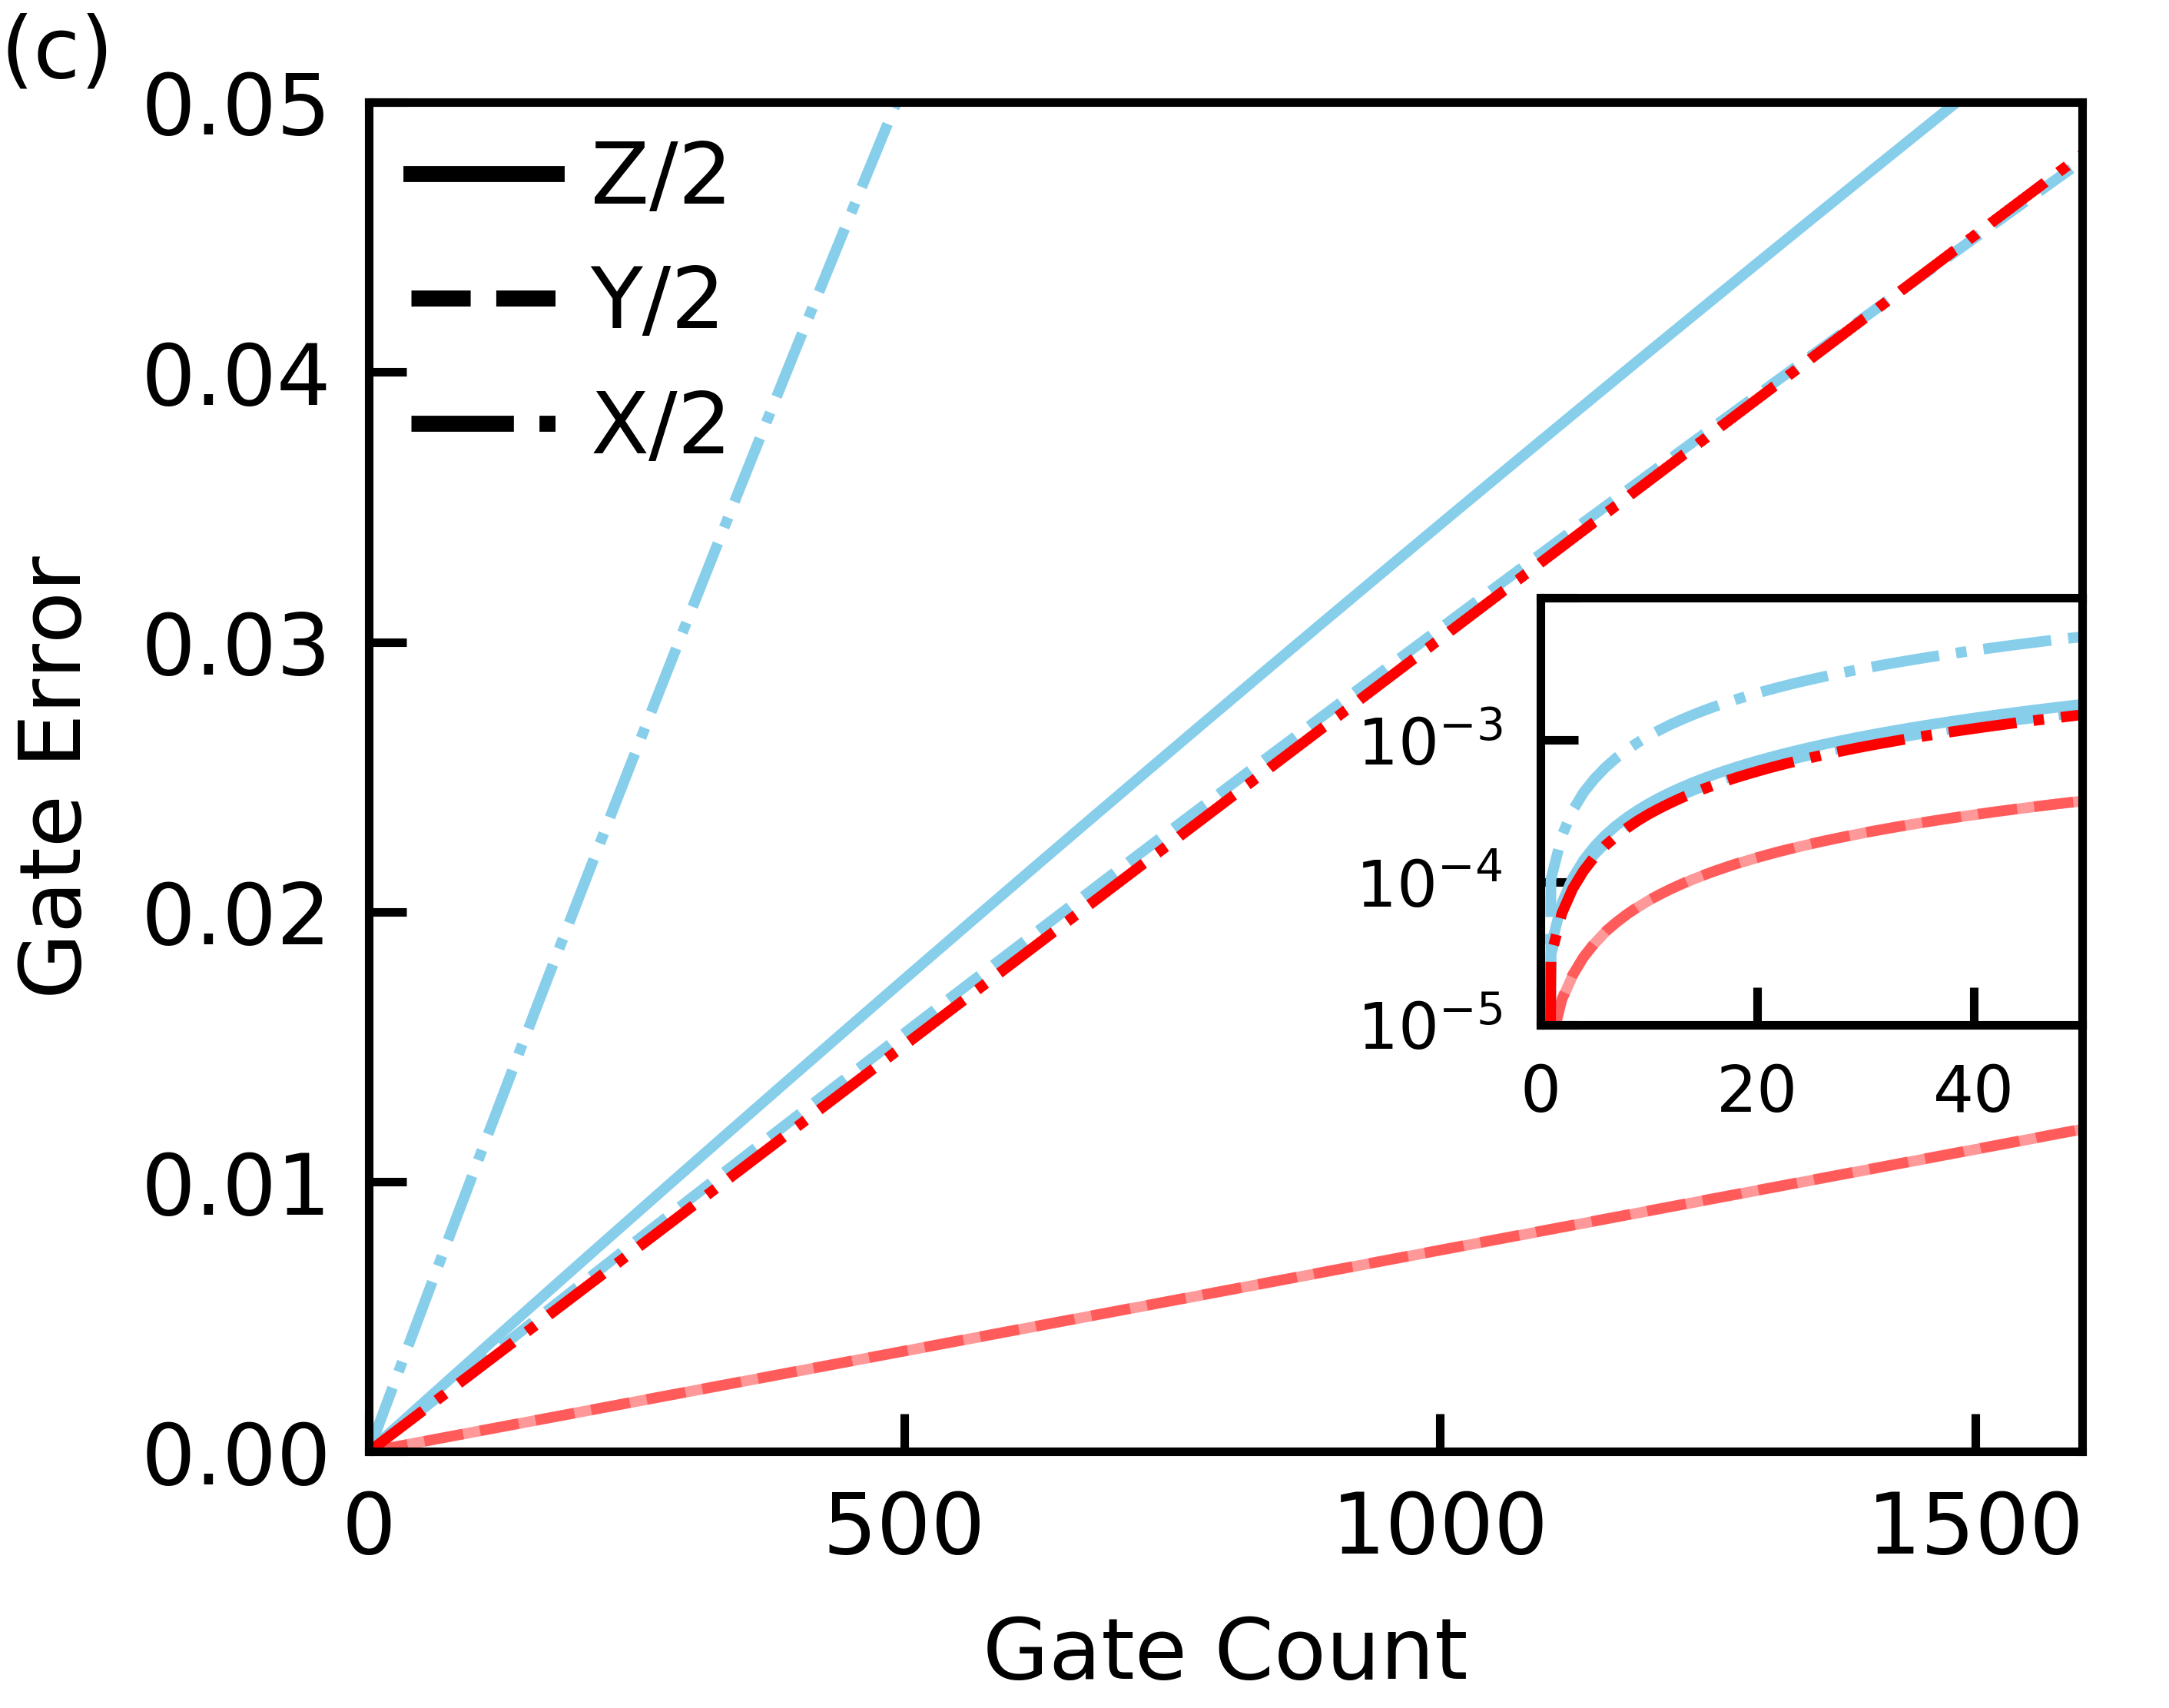
\includegraphics[width=\linewidth]{assets/f1c.png}
    \caption{\label{fig:longitudec}}
  \end{subfigure}
  \caption{
    (a) Numerically optimized gates (dark blue)
    and analytically optimized gates (light pink).
    (b) $T_{1}$ interpolation function used in optimization. Markers
    denote the time-averaged, absolute amplitude of each gate.
    (c) Cumulative gate errors due to depolarization as a function of the
    number of gates applied.
    Gate errors for the numerically optimized $Z/2$ and $Y/2$ gates
    are indistinguishable. Inset shows the cumulative gate errors
    plotted on a log scale for small gate counts.
  }
  \label{fig:longitude}
\end{figure*}

Next, we outline the cost functions for the fluxonium gate problem.
The augmented state and augmented control are:
\begin{equation}
  \begingroup
  \renewcommand*{\arraystretch}{1.3}
  x_{k} = \begin{bmatrix} \ket{\psi^{0}_{k}} \\ \ket{\psi^{1}_{k}}
    \\ \int_{t} a_{k} \\ a_{k} \\ \partial_{t} a_{k} \end{bmatrix} \quad
  u_{k} = \begin{bmatrix} \partial^{2}_{t} a_{k} \end{bmatrix}
  \endgroup
  \label{eq:astatecontrols}
\end{equation}
The cost function at each knot point is
$\ell_{k}(x_{k}, u_{k}) = (x_{k} - x_{f})^{T} Q_{k} (x_{k} - x_{f}) + u^{T}_{k} R_{k} u_{k}$
where $Q_{k}$ and $R_{k}$ are matrices we supply, and
$x_{f}$ is given by the constraints we have imposed on
$\ket{\psi^{i}_{N}}$, $\int_{t} a_{N}$, and $a_{N}$ in addition to
$\partial_{t} a_{f} = 0$. We choose $Q_{k}$ to be diagonal
so the cost function incentivizes the achievement of the constraints on
$\ket{\psi^{i}_{N}}$, $\int_{t} a_{N}$, and $a_{N}$,
and penalizes the norm of $\partial_{t} a_{k}$ and $\partial^{2}_{t} a_{k}$,
mitigating AWG ringing due to high-frequency transitions.
In the discrete dynamics function for this problem \eqref{eq:dyn_con},
we integrate the states according to the TDSE \eqref{eq:tdse} and the
fluxonium Hamiltonian \eqref{eq:hamiltonian} and integrate
the second-derivative of the flux amplitude to obtain
the first-derivative, proportional, and integral moments.
Stated succinctly, the optimization problem takes the form:
\begin{mini!}[2] 
  {x_{1:N}, u_{1:N\text{-}1}}{\sum_{k=1}^N {(x_k\text{-}x_f)}^{T} Q_k (x_k\text{-}x_{f})
    + \sum_{k=1}^{N-1} {u_k}^{T} R_k u_{k}}{}{} \label{eq:costfun}
  \addConstraint{x_{k+1}}{= f(x_k, u_k)}  \label{eq:dyn_con}
  \addConstraint{\ket{\psi^{0}_{1}} = \ket{0}, \ket{\psi^{1}_{1}} = \ket{1}} \label{eq:istate_con}
  \addConstraint{\ket{\psi^{i}_{N}} = U \ket{\psi^{i}_{1}}
    \ \forall \  i} \label{eq:tstate_con}
  \addConstraint{{\lvert \braket{\psi^{i}_{k}}{\psi^{i}_{k}}
      \rvert}^{2} = 1 \ \forall \ i, k} \label{eq:statenorm_con}
  \addConstraint{{\textstyle \int_{t}} a_{N} = 0} \label{eq:znf_con}
  \addConstraint{|a_{k}| \leq 0.5 \ \textrm{GHz} \ \forall \ k} \label{eq:amp_con}
  \addConstraint{a_{1} = a_{N} = 0} \label{eq:bound_con}
  \addConstraint{{\textstyle \int_{t}} a_{1} = \partial_{t} a_{1} = 0} \label{eq:ic_con}
\end{mini!}




